\section{Literature Review}
\label{sec:litreview}

I will provide an overview of some of the current research into automated redistricting algorithms, as well as compactness and partisan fairness measures. 

\subsection{Automated Redistricting Algorithms}

The purpose of automated redistricting algorithms is to generate a set of redistricting maps that are as "impartial" as possible \parencite{chen2013}. While many different algorithms have been proposed (see \textcite{altman2011}, \textcite{haas2020}, \textcite{lara-caballero2019}, \textcite{macmillan2001}, \textcite{weaver1963}, and \textcite{xiao2008}), I will provide high-level overviews of two algorithms: \hyperref[sec:smc]{Sequential Monte Carlo (SMC)} and \hyperref[sec:crsg]{Compact Random Seed Growth (CRSG)}. 

\subsubsection{Redistricting as Graph Cutting}
\label{sec:redistasgraphcut}


The following redistricting algorithms, SMC and CRSG, both conceptualize redistricting precincts as a graph-cutting problem. A graph is a network of different interconnected points, where the points are "nodes" and the lines connecting them "edges" \parencite{fifield2020}. Every precinct is a node, and geographically adjacent precincts have their corresponding nodes connected by edges. This is known as the "adjacency graph." Since the goal of redistricting is to assign every precinct to a district, the algorithms imagine that edges between nodes are "cut" until "islands" (known as "subgraphs") are formed, where each is disconnected from the others. The disconnected subgraphs then become the districts. See Figure \ref{fig:graphcut} for a visualization \parencite{fifield2020}. 

\begin{figure}[t]
    \caption{Redistricting as Graph Cutting}
    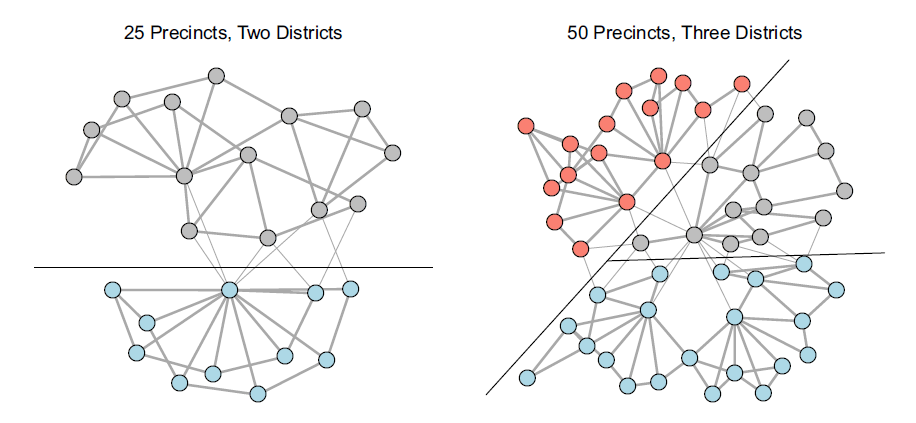
\includegraphics[width=0.7\linewidth]{img/graphcut.png}
    \label{fig:graphcut}
    \raggedright
    \figurenote{Every node is a precinct, and nodes that share an edge are known to be adjacent precincts. The algorithms "cut" edges between nodes until islands of districts are formed. \parencite[3]{fifield2020}}
\end{figure} 

\subsubsection{Sequential Monte Carlo (SMC)}
\label{sec:smc}

SMC is an implementation of the statistical method Sequential Monte Carlo\footnote{I use SMC to refer to the algorithm, not the statistical method.} \parencite{mccartan2020}. SMC views redistricting as a graph-cutting problem, but instead of the adjacency graph, it begins with a spanning tree, a graph with the fewest number of edges required to connect every node. If any individual edge is removed, 2 subgraphs are formed. 

\begin{figure}[hb]
    \caption{SMC Splitting Procedure}
    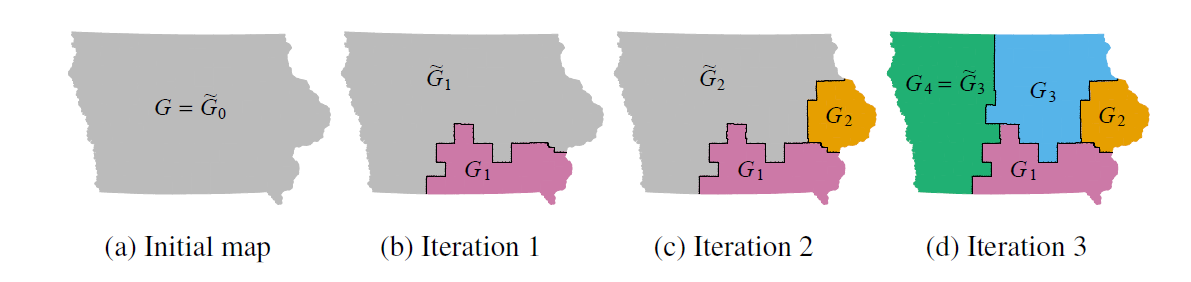
\includegraphics[width=\linewidth]{img/smc.PNG}
    \label{fig:smc}
    \raggedright
    \figurenote{One edge is chosen to be cut probabilistically, and the smaller resulting subgraph becomes a district if it satisfies the requirements. The procedure is repeated with the remaining subgraph until the desired number of districts are formed. \parencite[14]{mccartan2020}}
\end{figure}

Figure \ref{fig:smc} visualizes the iterative splitting procedure used by SMC. First, it computes the deviation from the target precinct population for each subgraph generated by cutting each edge in the spanning tree. Then, it randomly cuts one of the edges, creating two subgraphs. If the smaller subgraph meets the population and compactness requirements, then it's accepted as the first district, and the splitting procedure is repeated with the other subgraph. This process generates the possible redistricting maps that satisfy the requirements\footnote{For more details, please refer to \textcite{mccartan2020}.}.

\subsubsection{Compact Random Seed Growth (CRSG)}
\label{sec:crsg}

The following is a high-level overview of the CRSG algorithm\footnote{For more details, please see \textcite{chen2013}.}. 

CRSG begins by declaring that every precinct is it's own district. A random precinct is chosen and is merged with its closest neighboring precinct, creating one fewer district. This process is repeated until the desired number of districts are formed. \parencite{chen2013}

After this procedure, the districts are relatively compact due to the geographic proximity requirement, but there is no guarantee that the districts satisfy the equal population requirement. To satisfy the population parity requirements, CRSG does the following. First, it identifies the two adjacent districts that have the greatest difference in total population. Then the precinct in the more populous district that is furthest from the center of said district is reassigned to the less populous district, provided that this reassignment doesn't split either district into parts. This process is repeated until all of the districts are within some desired percentage of the mean district population. \parencite{chen2013}

One run of CRSG will produce one set of districts, and separate runs of CRSG with the same input data may produce slightly different districts \parencite{chen2013}.

\subsection{Compactness Measures}

A universal requirement of districts is that they be "reasonably compact." There is no single legal nor scholarly definition of compactness \parencite{katz2020}. The following is a brief overview of several different, commonly used compactness measures that have varying approaches, advantages, and weaknesses.

\subsubsection{Polsby-Popper Score}
\label{sec:polsbypopper}

\textcite{polsby1991} introduces the Polsby-Popper score, first developed in paleontology, to the problem of gerrymandering. It computes the ratio of the area of the district to the area of a circle with the same perimeter as the district \parencite{cox1927,polsby1991}. It ranges from 0 to 1, where 1 is most compact \parencite{polsby1991}.

Limitations and criticisms of this measure include that it is very sensitive to both geography and map resolution. Particularly near coastlines, even the most compact districts can have Polsby-Popper scores that are lower than gerrymandered districts which don't border coastlines. At finer resolutions, the same district will have a lower Polsby-Popper score as the perimeter increases. \parencite{mccartan2020}.

\subsubsection{Edge-Cut Compactness}
\label{sec:edgecut}

Edge-cut compactness takes a graph theory perspective to district compactness. The edge-cut compactness score is the number of edges that must be "cut" from the original adjacency graph to form the subgraphs, or districts \parencite{dube2016}. Theoretically, more-compact districts will require fewer edges to be cut \parencite{dube2016}. When normalized to the number of edges and subtracted from 1, a score of 1 indicates the most compact district. 

Benefits of this measure include that it is unaffected by political and natural geography, map resolution, and population density \parencite{mccartan2020}. 

\subsection{Partisan Fairness Measures}

\subsubsection{Seats-Votes Curve}
\label{sec:seatsvotes}

Seats-votes curves have been used to assess district maps for more than 40 years, and they are broadly supported in the literature \parencite{katz2020}. Seats-votes curves plot the relationship between the popular vote and the power balance in a legislature (or delegation). This plot has $V$, the average district-level proportion of votes won by Democrats (DVS), on the x-axis, and $S(V)$, the proportion of seats won by Democrats, on the y-axis \parencite{tufte1973}. Figure \ref{fig:seatsvotes} illustrates several hypothetical seats-votes curves.

\begin{figure}[hb]
    \caption{Types of Seats-Votes Curves}
    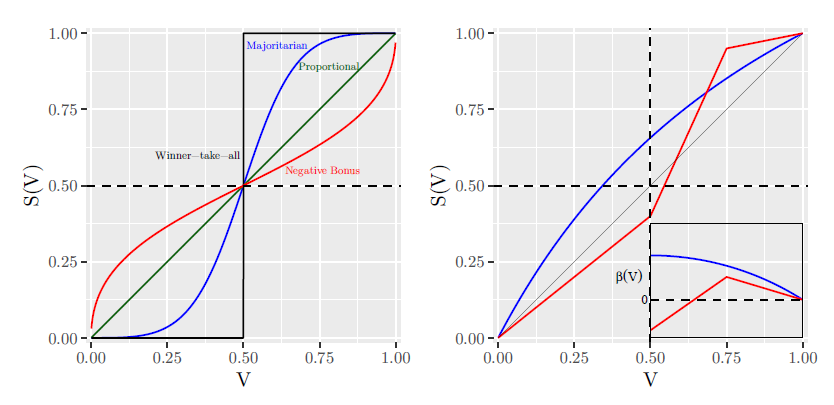
\includegraphics[width=0.6\linewidth]{img/seatsvotes.png}
    \label{fig:seatsvotes}
    \raggedright
    \figurenote{"Left panel: Symmetric (fair) curves with differing levels of electoral responsiveness Right panel: Asymmetric (biased) curves, including one consistently biased toward the Democrats (blue) and one with biases favoring different parties depending on V (red); the inset graph is for (V ) for V 2 [0:5; 1] with the vertical axis scaled to be the same as the main plot, and lines color coded to the seats-votes curves." \parencite[175]{katz2020}}
\end{figure}

It's very rare to observe sufficient electoral outcomes under the same electoral system in order to plot the complete curve (i.e., it's unlikely to observe DVS from 0 to 1 in separate elections occuring in the same districts). In practice, one can estimate a seats-votes curve using the uniform partisan swing principle \parencite{tufte1973}.

Uniform partisan swing is the principle that, when the DVS changes by some amount between elections, the individual vote share at the district level also changes by the same amount \parencite{tufte1973}. \textcite{katz2020} empirically verified this to be true in 646 different elections. 

Thus, given a list of district-level Democratic vote proportions from one election, one can adjust each vote proportion by an arbitrarily small amount until the entire seats-votes curve is computed \parencite{katz2020}.

The benefit of seats-votes curves is that they allow a complete view of the biases of a district map across all possible average district votes \parencite{gelman1994}. Unfortunately, generating these curves for one electoral map requires the use of statistical assumptions such as uniform partisan swing, as the number of elections occurring under a since district map is usually prohibitively small \parencite{warrington2018}.

Seats-votes curves visually represent the principles of partisan symmetry and partisan bias.

\paragraph{Partisan Symmetry}

A legislature (or delegation) exhibits partisan symmetry if both parties can receive $m$ proportion of the overall votes and therefore have $n$ proportion of the seats \parencite{katz2020}. If Republicans win 60\% of the votes but control 65\% of the seats, in a symmetrical system, Democrats should also be able to control 65\% of the seats by winning 60\% of the votes. Seats-votes curves that are rotationally-symmetrical about the center exhibit partisan symmetry \parencite{tufte1973}.

\paragraph{Partisan Bias}
\label{sec:bias}

Partisan Bias is the deviation from partisan symmetry in a tied election. If Democrats win 50\% of the average district vote but only win 40\% of the seats, there is a partisan bias of -0.1. Seats-votes curves that do not intersect the point $(0.5, 0.5)$ (the center) exhibit partisan bias \parencite{katz2020}.

\subsubsection{Single-Valued Fairness Measures}

The following measures compute a single value to assess the partisan fairness of a redistricting map and are actively disputed by areas of the literature.

\paragraph{Efficiency Gap}
\label{sec:effgap}

The efficiency gap is the difference between the number of wasted votes for each party, normalized to the total number of votes, where "wasted votes" are all votes for losing candidates and all votes for winning candidates over the 50\%-plus-one threshold. Theoretically, wasted votes are a sign of "packing" or "cracking," where a gerrymandered district intentionally groups voters together into the same district or dilutes their political power across several districts. \parencite{stephanopoulos2015}

\textcite{veomett2018} found that the efficiency gap is not a measure of partisan symmetry, as the measure becomes confused in highly non-competitive elections (e.g. party wins 80\% of the vote and 100\% of the seats). 

\paragraph{Declination}
\label{sec:declination}

Declination is another proposed measure of partisan asymmetry that "...relies only on the fraction of seats each party wins in conjunction with the aggregate vote each party uses to win those seats" \parencite[3]{warrington2018}. Broadly, it measures the declination in the line connecting the average vote proportions of one party in districts controlled by the other party \parencite{warrington2018}. See Figure \ref{fig:dec} for a visualization. 

\begin{figure}[b]
    \caption{Sample Declination Plots}
    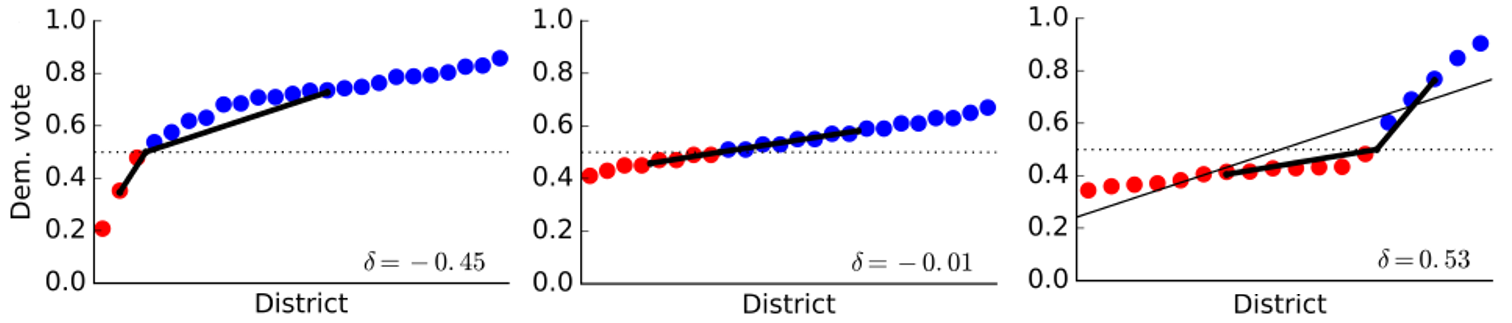
\includegraphics[width=0.8\textwidth]{img/dec.PNG}
    \label{fig:dec}
    \raggedright
    \figurenote{Districts plotted by ascending Democratic vote proportion. $\delta \approx 0$ is fair, $\delta < 0$ favors Democrats, and $\delta > 0$ favors Republicans. \parencite[6]{warrington2018}}
\end{figure}

\textcite{katz2020} refutes the claim of \textcite{warrington2018} that declination is a measure of partisan symmetry but acknowledges that it is a useful measure of the skewness of the distribution of district vote proportions. 

\subsubsection{Mean-Median Difference}
\label{sec:meanmed}

The mean-median difference is the difference between the mean and median DVS (first proposed by \textcite{mcdonald2015}). A mean-median difference of 0 indicates fair districts. 

\textcite{katz2020} finds that the mean-median difference is a reliable estimator of partisan bias only in highly competitive elections, when the average DVS is close to 0.5 \parencite{katz2020}.